\section{Atmoverb}

Si conclude infine con la progettazione del riverbero \emph{Atmoverb},
utilizzando le conoscenze maturate finora.

Il riverbero, come detto in precedenza, ha parametri di controllo relativi alle
condizioni atmosferiche dello spazio circostante. \todo{Circostante a cosa?}
Gli algoritmi di base utilizzati saranno i medesimi implementati in precedenza:
\emph{Comb} con \emph{Low-Pass} (figura \ref{fig:amcombfir}) e
\emph{All-Pass lattice} (figura \ref{fig:amapfo})

I parametri di controllo Temperatura, Pressione, Umidità, Gas

\begin{code}
atm = hslider("Pressure", 1, 0.1, 10, .1);
press = 76 * (atm);
temp = hslider("Temperature", 20, -200, 200, .1);
stp = (1.2930, 0.7710, 1.2507, 3.2170, 1.9760, 0.0899, 0.7170, 1.2500,1.4290, 0.804);
dens = (ba.take(1,stp)*press)/(press * (1 + (0.00367* (temp))));
velSuono = sqrt((1.402*atm*(1.013*10^5))/dens);
\end{code}

\todo{mancano i commenti e manca un process che faccia capire a cosa serve il
      codice. il senso di avere i blocchi separati viene meno se non funzionano
      autonomi e se non ci sono i commenti}

Viene così definita la velocità del suono che in seguto influenza i tempi di
Delay dei vari Comb, in base alla posizione del suono nello spazio.

\begin{code}
x = hslider("x",.5,.1,.99,.001);
y = hslider("y",.5,.1,.99,.001);
z = hslider("z",.15,.1,.99,.001);

Dim = hslider("Room Dimension",1,1,100,.1);

altezza = 3*Dim;
larg = 3*Dim;
lung = 6*Dim;
\end{code}

\todo{idem}

Le variabili x, y, z servono per identidficare il punto di origine dell'evento sonoro, scalate
per Dim in modo da rendere variabile la dimensione della stanza.

I coefficenti di assorbimento delle pareti sono stati inseriti anch'essi, in quanto sappiamo
avere una certa influenza sul risultato sonoro. I valori sono compresi tra 0
(completamente assorbente) e 1 (completamente riverberante). I valori sono stati decisi
arbitrariamente per simulare una sala da concerto (il pavimento è il valore più basso per
l'influenza delle sedute).

\begin{code}
rifLat = .8;
rifFro = .5;
rifSoff = .85;
rifPav = .3;
\end{code}

Dato che il riverbero utilizza un'architettura Comb-AllPass, avente quindi diversi valori di g e di t
per i vari comb, calcoliamo i coefficenti utilizzando le variabili descritte prima.

\bigskip

Tempi:
\begin{code}
t1 = ((z*altezza)/velSuono);
t6 = (((1 - z)*altezza)/velSuono);
t2 = ((x*larg)/velSuono);
t3 = (((1 - x)*larg)/velSuono);
t4 = ((y*lung)/velSuono);
t5 = (((1 - x)*lung)/velSuono);

ts = (t1, t6, t2, t3, t4, t5);
tsa1 = (t1,t2,t4);
tsa2 = (t6,t3,t5);
\end{code}

Gain
\begin{code}
gs1 = z*rifPav ;
gs6 = (1 - z)*rifSoff ;
gs2 = x*rifLat;
gs3 = (1 - x)*rifLat;
gs4 = y*rifFro ;
gs5 = (1 - y)*rifFro ;

gs=(gs1,gs6,gs2,gs3,gs4,gs5);
gsa1=(gs1,gs2,gs4);
gsa2=(gs6,gs3,gs5);
\end{code}

I valori di g e t sono stati divisi a loro volta in 2 liste separate in modo tale da gestire
il segnale tra 2 canali ed avere un minimo di spazializzazione.

Il risultato finale è

\begin{code}
process = _,_<:((_<:*(1-g)+(_<: par(i,3,dfldf(ba.take(i+1,tsa1),g,ba.take(i+1,gsa1))) :>
seq(i,2,apfo(2,T, g)))/2) ,(_<:*(1-g)+(_<: par(i,3,dfldf(ba.take(i+1,tsa2),g,ba.take(i+1,gsa2))) :>
seq(i,2,apfo(2,T, g)))/2) ) ;
\end{code}

\begin{figure}[htp]
\centering
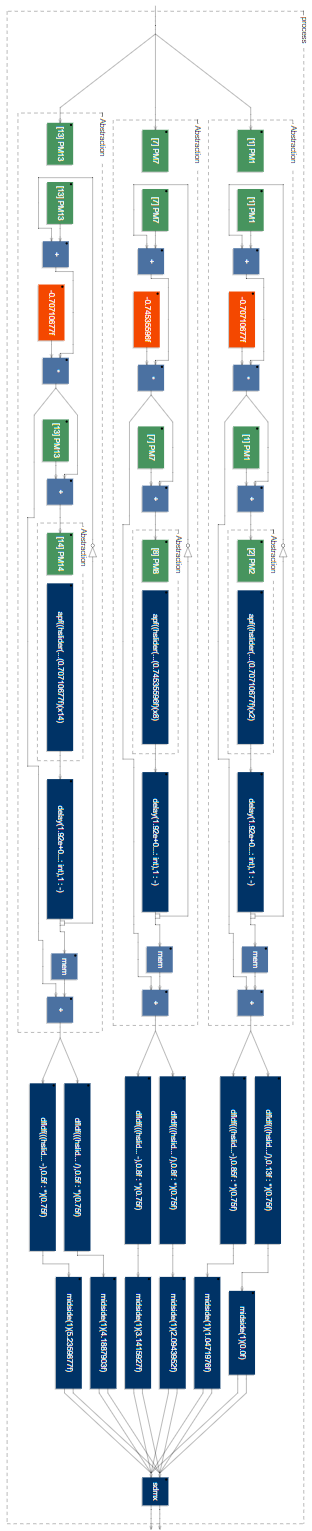
\includegraphics[width=1\textwidth]{atmoverb}
\label{fig:atmoverb}
\end{figure}

\todo[inline]{il codice preso a blocchi e rimesso insieme in un process non funziona. non so cosa fare e come aiutarti}
